%=================================================================
% fp-tools BioMedInformatics manuscript
% Compile with: latexmk -pdf main.tex   (or pdflatex x3)
% Requires the MDPI class shipped under Definitions/ (extracted from
% paper/MDPI_template_ACS.zip by paper/scripts/prepare_biomedinformatics_template.py)
%=================================================================
\documentclass[biomedinformatics,article,submit,pdftex,moreauthors]{Definitions/mdpi}

% MDPI internal commands - do not modify
\firstpage{1}
\makeatletter
\setcounter{page}{\@firstpage}
\makeatother
\pubvolume{1}
\issuenum{1}
\articlenumber{0}
\pubyear{2026}
\copyrightyear{2026}
\datereceived{ }
\dateaccepted{ }
\datepublished{ }

%------------------------------------------------------------------
\Title{fp-tools: A Reproducible Command-Line Platform for Classical and
Multiscale ATAC-seq Footprinting, Motif Discovery Preparation, Pseudobulk
Aggregation, and Replicate-Aware Reporting}

\Author{Yaoxiang Li $^{1}$ and Chunling Yi $^{1,}$*}

\AuthorNames{Yaoxiang Li and Chunling Yi}

\address{%
$^{1}$ \quad Department of Oncology, Lombardi Comprehensive Cancer Center, Georgetown University Medical Center, Georgetown University, Washington, DC, USA; yl814@georgetown.edu (Y.L.); cy232@georgetown.edu (C.Y.)}

\corres{Correspondence: cy232@georgetown.edu (C.Y.)}

\abstract{(1) Background: Transcription-factor (TF) footprinting from ATAC-seq is
central to inferring regulatory activity, but the surrounding ecosystem is
fragmented across single-purpose tools with heterogeneous interfaces,
inconsistent reproducibility, and uneven test coverage, which raises the cost of
building end-to-end regulatory-genomics analyses. (2) Methods: We present
\texttt{fp-tools}, a standalone, pip-installable Python package that unifies bias
correction, footprint scoring, differential TF-binding detection, and aggregate
visualization in a reproducible command-line package. Around this core we add
first-version utilities for multiscale and nucleosome-aware scoring, de novo
motif-discovery preparation, single-cell pseudobulk aggregation, and
replicate-aware differential-binding reporting. (3) Results: The package provides deterministic,
regression-tested workflows, reproducible figure generators, and a tiered
public-data benchmark design for the supported first-version workflow. Existing
classical analyses remain unchanged when optional utilities are not invoked. (4) Conclusions: \texttt{fp-tools} integrates
established footprinting strengths with pragmatic multiscale, replicate-aware,
pseudobulk, and motif-discovery helper utilities in a single reproducible package,
lowering the barrier to standardized, benchmarkable ATAC-seq regulatory analysis.}

\keyword{ATAC-seq; transcription factor footprinting; chromatin accessibility;
motif analysis; multiscale footprints; pseudobulk ATAC-seq;
replicate-aware reporting; reproducibility; command-line bioinformatics}

% Use an external BibTeX database (references.bib) with the MDPI style.
\externalbibliography{yes}

\begin{document}

%==================================================================
\section{Introduction}
%==================================================================

Chromatin accessibility profiling by the assay for transposase-accessible
chromatin using sequencing (ATAC-seq) has become a standard readout of the active
regulatory landscape of a cell~\cite{buenrostro2013}. Within accessible regions,
sequence-specific transcription factors (TFs) protect the DNA they occupy from
transposition, leaving characteristic depletions---``footprints''---flanked by
hyper-accessible edges. Detecting and interpreting these footprints supports
inference of TF occupancy, differential regulation between conditions, and the
functional consequences of non-coding variation.

A mature but \emph{fragmented} ecosystem of methods addresses pieces of this
problem. Classical footprinting and differential-binding frameworks such as
TOBIAS~\cite{bentsen2020} and HINT-ATAC~\cite{li2019hint} correct enzymatic
sequence bias and score footprints at a single TF-relevant scale. Multiscale and
nucleosome-aware approaches, exemplified by the PRINT/scPrinter
family~\cite{hu2024print}, model accessibility structure across a range of
footprint widths. Supervised TF-binding-site (TFBS) predictors such as
maxATAC~\cite{cazares2023maxatac} and sequence-to-profile models such as
ChromBPNet~\cite{chrombpnet2024} learn occupancy from labeled data or raw
sequence, and downstream interpretation tools and variant scorers translate models
into motif and allele-level effects. Each tool typically ships its own interface,
input conventions, and assumptions, so assembling a coherent, reproducible
pipeline---and \emph{benchmarking} alternatives on common ground---remains
laborious and error-prone.

Beyond this tooling friction, footprint interpretation has practical limitations
that make reproducibility and careful signal handling important. Classical
footprinting depends on base-resolution cut-site depletion and can be confounded
by enzyme sequence bias, local accessibility, motif strength, and factor-specific
binding kinetics~\cite{sung2014}. Deep sequence-to-profile models and multiscale
methods can improve sensitivity for some questions, but they often require
substantial compute and specialized training workflows. For many applied ATAC-seq
projects, the immediate need is therefore a transparent, repeatable workflow that
keeps the classical analysis reliable while exposing selected extensions without
forcing users into a different software ecosystem.

Four gaps motivate this work. First, \textbf{signal clarity}: users need to know
which signal representation is appropriate for footprint scoring and how optional
normalization changes interpretation. Second, \textbf{interface fragmentation}:
moving from bias correction to footprint scoring to differential binding to
visualization commonly spans several packages with incompatible I/O. Third,
\textbf{reproducibility and testing}: many footprinting workflows lack
deterministic regression tests, pinned environments, and machine-checkable output
contracts, making it hard to know whether a change altered results. Fourth,
\textbf{extensibility without regression}: adding new scientific behavior, such
as multiscale scoring or pseudobulk aggregation, should not destabilize the
classical workflow.

We address these gaps with \texttt{fp-tools}, a reproducible ATAC-seq
footprinting platform that keeps the classical workflow intact while adding a
small set of practical first-version utilities. The package unifies bias
correction, footprint scoring, motif-aware differential binding, and aggregate
visualization, then extends this core with multiscale scoring, de novo
motif-discovery preparation, pseudobulk ATAC aggregation, and replicate-aware
reporting. The goal is not to replace specialized deep-learning or variant-scoring
systems in this first version, but to make a complete footprinting analysis easier
to run, audit, repeat, and benchmark. This paper describes the supported methods,
tiered validation design, and reproducibility engineering that tie these workflows
together.

%==================================================================
\section{Materials and Methods}
%==================================================================

\subsection{Package Architecture and Core Workflows}

\texttt{fp-tools} is distributed as a pip-installable package (\texttt{fp-tools-bio})
with vendored Cython internals for performance-critical signal operations. The
core workflow has four method layers: Tn5 sequence-bias correction, footprint
scoring over corrected signal, motif-anchored differential TF-binding analysis,
and aggregate visualization around TFBS or region sets. These layers share common
region, signal, motif, and sample-label conventions so intermediate files can be
passed through a complete analysis without format-specific glue code. YAML
configuration files provide a reproducible way to save and rerun the same analysis
without changing the underlying methods.

For classical footprint scoring, let $x_i$ denote corrected Tn5 cut-site signal
around candidate position $p$. The default footprint score is a center-versus-flank
contrast,
\[
F(p)=\frac{1}{|L|+|R|}\left(\sum_{i\in L}x_i+\sum_{i\in R}x_i\right)-
\frac{1}{|C|}\sum_{i\in C}x_i,
\]
where $C$ is the protected center and $L$ and $R$ are flanking windows. Larger
values therefore correspond to the expected footprint pattern: fewer cuts at the
putative bound site and more cuts in nearby accessible flanks.

The multiscale module generalizes this single-scale contrast to a set of footprint
widths $\mathcal{S}$. For a scale $s$, the center, left, and right windows
$C_s(i)$, $L_s(i)$, $R_s(i)$ are sized to $s$, giving a scale-specific depletion
\[
F_s(i)=\frac{1}{|L_s(i)|+|R_s(i)|}\left(\sum_{j\in L_s(i)}x_j+\sum_{j\in R_s(i)}x_j\right)-
\frac{1}{|C_s(i)|}\sum_{j\in C_s(i)}x_j,
\]
collapsed to a per-position summary by either the maximum or the mean over scales,
\[
F_{\max}(i)=\max_{s\in\mathcal{S}}F_s(i),\qquad
F_{\mathrm{mean}}(i)=\frac{1}{|\mathcal{S}|}\sum_{s\in\mathcal{S}}F_s(i).
\]
The full scale-by-position matrix $\{F_s(i)\}$ is retained in the NPZ tensor
sidecar, so narrow TF-scale and broader nucleosome-scale structure can be
evaluated in the same regions.


\subsection{First-Version Opt-in Utilities}

New behavior is added as explicit optional utilities, each inert unless selected:
\begin{itemize}
  \item \emph{Multiscale and nucleosome-aware scoring} computes depletion across a
        configurable set of window sizes (default 8--147~bp), collapses the
        scale-specific scores by maximum or mean, and can retain the full
        scale-by-position tensor for downstream visualization.
  \item \emph{De novo motif-discovery preparation} exports candidate-centered
        sequences, records reproducible MEME/DREME~\cite{bailey2015meme} and
        Tomtom~\cite{gupta2007tomtom} settings, and summarizes discovered motifs
        and matches to known motif databases. This can be run as a standalone
        discovery step or as a supplement to known-motif analyses when a database,
        such as a JASPAR release, may not contain all active motifs in the sample.
  \item \emph{Pseudobulk aggregation} groups single-cell ATAC fragments by
        annotation columns into bulk-like fragment files, manifests, optional
        indexed outputs, and optional normalized cut-site tracks for downstream
        footprinting and aggregate plots.
  \item \emph{Replicate-aware differential binding} treats repeated samples from
        the same condition as biological replicates, reports condition means and
        replicate variation, and produces diagnostic tables and figures for
        differential TF-binding comparisons (Section~\ref{sec:replicate}).
\end{itemize}

Conceptually, the first-version utilities answer focused questions around the
classical core. Multiscale scoring asks whether depletion occurs only at a narrow
TF-like width or also at broader nucleosome-consistent widths; de novo motif
preparation asks which sequence patterns recur among exported candidate sites;
replicate-aware reporting asks whether repeated-condition inputs can be summarized
as condition means and replicate variation; and pseudobulk aggregation asks
whether single-cell fragments can be grouped into interpretable group-level
profiles that run through the same footprinting machinery. In this work we validate that path
with a public 10x Genomics PBMC Multiome dataset processed by Cell Ranger ARC
2.0.0~\cite{tenxpbmc2021}. Official 10x gene-expression graph clusters are
collapsed into broad PBMC labels using canonical marker-gene enrichments (B cells,
CD4 T cells, NK/cytotoxic T cells, CD14 monocytes, FCGR3A monocytes, dendritic
cells, and mixed myeloid cells), then ATAC fragments are split by label and
converted to CPM-normalized cut-site bigWigs. Motif-associated peak sets for PAX5,
TCF7/TCF7L2, CEBPB, and CTCF are taken from the 10x TF-analysis peak--motif
mapping distributed with the same dataset.

\subsection{Replicate-aware Differential Binding and Quantile Normalization}
\label{sec:replicate}

Replicate-aware analysis is integrated directly into \texttt{detect-tf-binding}.
If users pass repeated condition names, for example
\texttt{--cond-names Bcell Bcell Tcell Tcell}, fp-tools treats the corresponding
signal files as biological replicates of the same condition while preserving the
original BINDetect-style output columns. Let $x_{c,r,i}$ be the footprint score at
site or background position $i$ for replicate $r$ of condition $c$. With
\texttt{--normalization sample-quantile}, each replicate is normalized before
condition averaging using the same BINDetect-style multiplicative quantile curve
used throughout fp-tools. For sample $s$, fp-tools computes empirical positive
score quantiles $q_s(p)$ and the reference quantile
$q_\ast(p)=S^{-1}\sum_s q_s(p)$ across the $S$ input samples, then fits a smooth
multiplicative factor $g_s(x)$ to the ratio $q_\ast(p)/q_s(p)$. Each score is
transformed as
\[
\tilde{x}_{s,i}=\max\{0,\,x_{s,i}g_s(x_{s,i})\}.
\]
The default \texttt{condition-quantile} mode preserves the previous behavior by
first averaging replicate background distributions within each condition, fitting
one factor $g_c(x)$ per condition, and applying that condition-level factor to
all replicates in the condition before final condition means and SDs are reported;
\texttt{none} disables this step. The same shared normalization helper and the
same sample-first versus condition-first ordering are used by
\texttt{plot-aggregate}, so aggregate visualizations and
\texttt{detect-tf-binding} comparisons are normalized consistently. Because this
step removes distribution-level depth and background offsets, differential
interpretation is based on normalized per-site contrasts and the BINDetect
comparison statistic, not on global baseline height alone.

After normalization, condition-level scores are summarized as
\[
\bar{x}_{c,i}=\frac{1}{n_c}\sum_{r=1}^{n_c}\tilde{x}_{c,r,i},\qquad
s_{c,i}=\sqrt{\frac{1}{n_c-1}\sum_{r=1}^{n_c}(\tilde{x}_{c,r,i}-\bar{x}_{c,i})^2}.
\]
For a comparison between conditions $c_1$ and $c_2$, fp-tools reports both an
interpretable footprint-score difference and a stabilized log fold change,
\[
\Delta_i=\bar{x}_{c_1,i}-\bar{x}_{c_2,i},\qquad
L_i=\log_2\frac{\bar{x}_{c_1,i}+\epsilon}{\bar{x}_{c_2,i}+\epsilon},
\]
where $\epsilon$ is the BINDetect pseudocount estimated from the background signal
unless supplied explicitly. When both conditions have replicate support, approximate
standard errors are reported as
\[
\mathrm{SE}(\Delta)=\sqrt{\frac{s_1^2}{n_1}+\frac{s_2^2}{n_2}},
\]
\[
\mathrm{SE}(L)\approx\frac{1}{\ln 2}
\sqrt{\frac{s_1^2}{n_1(\mu_1+\epsilon)^2}+
      \frac{s_2^2}{n_2(\mu_2+\epsilon)^2}}.
\]
The original BINDetect standardized \texttt{change} and \texttt{pvalue} columns
remain unchanged for compatibility. Additional columns include replicate counts,
condition score SDs, mean $\Delta$, mean $L$, and standard-error summaries. A
legacy replicate-report command remains available as a post-hoc helper for
existing \texttt{*\_results.txt} files.

\subsection{Public Data, Benchmark Tiers, and Metrics}

Benchmarks are organized as versioned TSV manifests recording source, benchmark
tier, cell type, donor, TF, assay, accessions, assembly, output type, format,
URL, checksum, status, local path, split, and notes. A discovery script queries
the ENCODE REST API for released human GRCh38 ATAC-seq and matched TF
ChIP-seq/CUT\&RUN; a resumable downloader writes per-benchmark download reports
with checksums and local paths. Raw and processed public data, and large
benchmark outputs, are kept out of version control; scripts, manifests, schemas,
tiny fixtures, and figure code are tracked.

The benchmark is deliberately \emph{tiered} rather than monolithic
(Table~\ref{tab:tiers}): a fast CI-smoke tier on tiny fixtures; a bulk matched
tier (ENCODE bulk ATAC vs. matched TF ChIP/CUT\&RUN) as the primary classical
benchmark; a depth-robustness tier over downsampled ATAC; a de novo motif-preparation tier;
and a real-data pseudobulk demonstration tier. For binary TF-binding labels we compute AUROC and
AUPRC globally and per TF-cell task, recall at 1\%, 5\%, and 10\% FDR, precision at
fixed recall, calibration curves with expected and maximum calibration error,
Brier score for probability models, per-TF macro averages, Wilcoxon signed-rank
tests for paired method comparisons, and stratified bootstrap confidence intervals
for key deltas. Expected calibration error partitions predictions into $B$
equal-width probability bins and averages the gap between confidence and accuracy,
\[
\mathrm{ECE}=\sum_{b=1}^{B}\frac{n_b}{n}\left|\mathrm{acc}(b)-\mathrm{conf}(b)\right|,
\]
with maximum calibration error defined analogously as the worst-bin gap. Metric, calibration, and bootstrap computations are implemented as
standalone, unit-tested scripts and combined by a benchmark pipeline runner that
also emits PDF/SVG/PNG figure panels.

\begin{table}[H]
\caption{Tiered benchmark design. Large data and outputs are untracked; only
manifests, scripts, and small smoke results are committed.\label{tab:tiers}}
\newcolumntype{Y}{>{\raggedright\arraybackslash}X}
\begin{tabularx}{\textwidth}{lYY}
\toprule
\textbf{Tier} & \textbf{Purpose} & \textbf{Primary outputs}\\
\midrule
CI smoke & Install/regression checks on tiny fixtures & command success, output existence, stable summaries\\
Bulk matched & Main classical benchmark (ATAC vs. matched TF ChIP/CUT\&RUN) & TFBS labels, predictions, AUROC/AUPRC, reports\\
Depth robustness & Shallow-depth sensitivity (50/25/10/5\%) & performance-vs-depth and calibration curves\\
De novo motif prep & Candidate FASTA and motif-discovery helper validation & exported FASTA, command plans, motif summaries\\
Pseudobulk & Single-cell extension and real-data demonstration & 10x PBMC cell-type pseudobulks, TF aggregate profiles\\
\bottomrule
\end{tabularx}
\end{table}

\subsection{Reproducibility Engineering}

The package ships a unit-test suite covering numerical helpers, CLI behavior, and
deterministic golden CLI regressions for footprint scoring, differential binding,
and aggregate plotting, with an opt-in slow regression for bias correction. A
continuous-integration workflow runs the suite on a clean checkout using only
small fixtures. Every benchmark result is expected to store random seeds, tool
versions, command lines, and the resolved manifest. Figures are saved as vector
PDF/SVG plus 300-dpi PNG previews, with source plotting tables retained for
auditability.

%==================================================================
\section{Results}
%==================================================================

\subsection{A Unified, Reproducible Footprinting Platform}

\texttt{fp-tools} consolidates the four core ATAC footprinting workflows behind a
single, consistent workflow with shared region/signal conventions, so a complete
analysis---bias correction, footprint scoring, differential binding, and aggregate
visualization---runs without crossing package boundaries or reformatting
intermediates. Optional YAML configuration records the same analysis in a
machine-readable form for reruns and batch processing (Figure~\ref{fig:workflow}).

\begin{figure}[H]

\includegraphics[width=\textwidth]{figures/fp-tools-workflow.png}
\caption{Overall \texttt{fp-tools} workflow. Bulk ATAC-seq inputs enter a
legacy-compatible classical core for Tn5 bias correction, footprint scoring,
TF-binding detection, and aggregate visualization. Optional YAML and batch layers record reproducible analyses, while first-version
utilities add multiscale scoring, de novo motif preparation, pseudobulk support,
and replicate-aware reporting. Outputs include
signal tracks, reports, motif summaries, pseudobulk manifests, benchmark metrics,
and reproducible paper-ready figures.\label{fig:workflow}}
\end{figure}

\subsection{Deterministic Regression and CLI Coverage}

The classical workflow is covered by deterministic golden regressions that pin
output summaries for footprint scoring, differential binding, and aggregate
plotting, plus smoke tests for public entry points and YAML dry-runs. This converts ``did this change alter results?'' from a manual judgment
into an automatically checked contract, and provides the stable base on which the
opt-in modules are layered without disturbing default behavior.

\subsection{Multiscale and Nucleosome-aware Extension}

The multiscale module augments single-scale footprint scoring with a
scale-by-position view of accessibility depletion. The compressed NPZ tensor
sidecar serves as a paper-figure input for scale-by-position visualization. On synthetic constructs, narrow TF-scale and broad
nucleosome-scale depletions are recovered at their respective scales, and the
companion aggregate visualization (scale-by-position heatmap, collapsed profile,
and per-scale means) renders these directly. Crucially, default single-scale
scoring is unchanged unless multiscale mode is requested.


\subsection{De Novo Motif Preparation}

The de novo motif-preparation path exports candidate-centered FASTA files,
constructs reproducible MEME/DREME and Tomtom analysis records, and summarizes
motif results into TSV/HTML reports with inline consensus logos. This keeps
external motif discovery reproducible without making a new motif-calling algorithm
part of the first-version claim. The workflow can be used alone to discover
recurring patterns in candidate intervals, or after known-motif scanning to find
additional motifs not represented in the selected database.

\begin{figure}[H]

\includegraphics[width=\textwidth]{figures/fp-tools-de-novo-motif.png}
\caption{De novo motif-discovery preparation workflow. Candidate-centered
sequences are exported from BED-like intervals, external MEME/STREME and Tomtom
runs are captured as reproducible command plans, and motif summaries are returned
as concise tables and reports. This first-version utility prepares reproducible
motif-discovery inputs and reports without claiming a new motif-calling
algorithm.\label{fig:denovo_motif_prep}}
\end{figure}

\subsection{Replicate-aware Normalization}

Replicate-aware \texttt{detect-tf-binding} adds an interpretable layer to
differential binding: repeated condition names define biological replicate groups,
condition means are reported alongside per-condition SDs, and optional
sample-level quantile normalization applies the same distribution-matching step
before replicate group averages are compared. To make the effect visible, we
used a real-track label-orientation demo built from ATF7-associated
corrected cut-site matrices. The upper panel reverses the B/T labels and is named
IRF4 as a B-cell-deeper example, whereas the lower panel keeps the original ATF7
orientation as a T-cell-deeper example. This keeps the footprint shape from real
corrected signal while showing that sample-level quantile normalization strongly
reduces raw baseline offsets and preserves the center-versus-flank depletion
direction (Figure~\ref{fig:normalization_effect}).

\begin{figure}[H]

\includegraphics[width=0.95\textwidth]{figures/normalization_effect.png}
\caption{Effect of sample-level quantile normalization on replicate-aware
corrected cut-site aggregate profiles. Real ATF7-associated corrected cut-site matrices were used in two label
orientations: an IRF4-named B-cell-deeper orientation with B/T labels reversed and
the original ATF7 T-cell-deeper orientation. Condition means are
shown with light replicate-variation ribbons. The right column uses the same nonnegative-clamped sample-quantile
normalization path used by replicate-aware \texttt{detect-tf-binding} and
\texttt{plot-aggregate}; raw baseline offsets are reduced and a lower center
relative to the local flanks indicates stronger TF protection.
Generated by
\texttt{paper/scripts/plot\_normalization\_effect.py}.}
\label{fig:normalization_effect}
\end{figure}

\subsection{Real 10x PBMC Pseudobulk Validation}

To test whether the pseudobulk utility supports mainstream single-cell ATAC data
rather than only toy fixtures, we ran \texttt{fp-tools-pseudobulk} on the public
10x Genomics PBMC granulocyte-sorted Multiome dataset~\cite{tenxpbmc2021}. The
workflow used the official 10x ATAC fragments and GEX graph clusters, mapped 11,898
cells into broad immune pseudobulks, and retained seven groups after requiring at
least 300 cells and 50,000 fragments: B cells, CD4 T cells, NK/cytotoxic T cells,
CD14 monocytes, FCGR3A monocytes, dendritic cells, and a mixed myeloid group. The
kept pseudobulks contained 13.6--144.0 million counted fragments per group and
were written as indexed fragment files plus CPM-normalized cut-site bigWigs. These
outputs were readable by the same aggregate-plotting code used for bulk ATAC data.

As a qualitative validation, we aggregated pseudobulk cut-site signal around 10x
motif-associated peak centers for immune-relevant TFs (PAX5, TCF7/TCF7L2, CEBPB,
and CTCF). The resulting multi-panel profile shows that the single-cell fragments
can be collapsed into interpretable group-level tracks and compared across immune
cell types without changing the downstream bulk-style visualization machinery
(Figure~\ref{fig:pseudobulk_supp}). This result is intended as a support and
reproducibility demonstration, not as a full single-cell benchmark.

\begin{figure}[H]

\includegraphics[width=\textwidth]{figures/supp_pseudobulk_tf_aggregates.png}
\caption{Real 10x PBMC pseudobulk TF aggregate profiles.
Single-cell ATAC fragments from the public 10x PBMC Multiome dataset were grouped
by broad immune-cell labels derived from official 10x gene-expression graph
clusters, converted to CPM-normalized cut-site bigWigs, and aggregated around
10x motif-associated peak centers for PAX5, TCF7/TCF7L2, CEBPB, and CTCF. The
figure demonstrates that \texttt{fp-tools-pseudobulk} produces group-level signal
tracks that can be visualized by the same aggregate-profile workflow used for bulk
ATAC data. Generated by \texttt{paper/scripts/plot\_pseudobulk\_tf\_aggregates.py}.
\label{fig:pseudobulk_supp}}
\end{figure}

\subsection{Benchmark and Figure Infrastructure}

The tiered benchmark design (Table~\ref{tab:tiers}), metric scripts, manifest
builders, and figure-generation scripts provide an executable path from public
inputs to publication-ready outputs. In the first-version scope, these resources
serve three purposes. First, they verify that the classical footprinting workflow
continues to produce stable outputs on small fixtures and public-data subsets.
Second, they provide matched-label scaffolds for bulk ATAC comparisons against
TF ChIP-seq or CUT\&RUN labels without making those scaffolds part of the
first-version user workflow.
Third, they support focused demonstrations for multiscale scoring, de novo
motif-preparation, pseudobulk aggregation, replicate-aware normalization, and
cut-site-resolution footprint scoring.

Each benchmark run is expected to write a resolved manifest, software versions,
parameters, and plotting tables next to the generated figures. This makes the
figures auditable: a reader can inspect which samples, motifs, regions, and signal
tracks were used, and a developer can rerun the same tier after code changes. The
same infrastructure can later support larger model-comparison studies, but those
studies are outside the current first-version claim.

\subsection{Footprinting Requires Cut-Site Resolution}

Footprinting infers occupancy from a local depletion of Tn5 insertions at the bound
site, flanked by hyper-accessible edges. We tested this directly on K562 CTCF
(chromosome~4) by computing a footprint-occupancy score at each peak's best CTCF
motif match---the mean signal in the flanks minus the mean signal at the motif
site---using two different signal representations
(Figure~\ref{fig:footprint}). On a smoothed fold-change-over-control coverage
track the score is uninformative and in fact inverted (AUROC $=0.24$), because
coverage is \emph{enriched}, not depleted, at bound accessible sites. When the same
score is computed from base-resolution Tn5 cut sites derived from the ATAC BAM, it
recovers a genuine footprint signal (AUROC $=0.68$, 95\% CI $0.65$--$0.70$)---a
large gain that arises purely from using the correct, cut-site-resolution signal
that \texttt{fp-tools}' bias-correction and footprint-scoring pipeline is built to
produce. For CTCF, whose long motif is already highly predictive, the cut-site
footprint is an orthogonal but weaker line of evidence and does not exceed the motif
score; footprinting is expected to contribute most where motifs are weak or where
condition-specific occupancy changes are the question, which the differential
binding and replicate-aware modules target.

\begin{figure}[H]
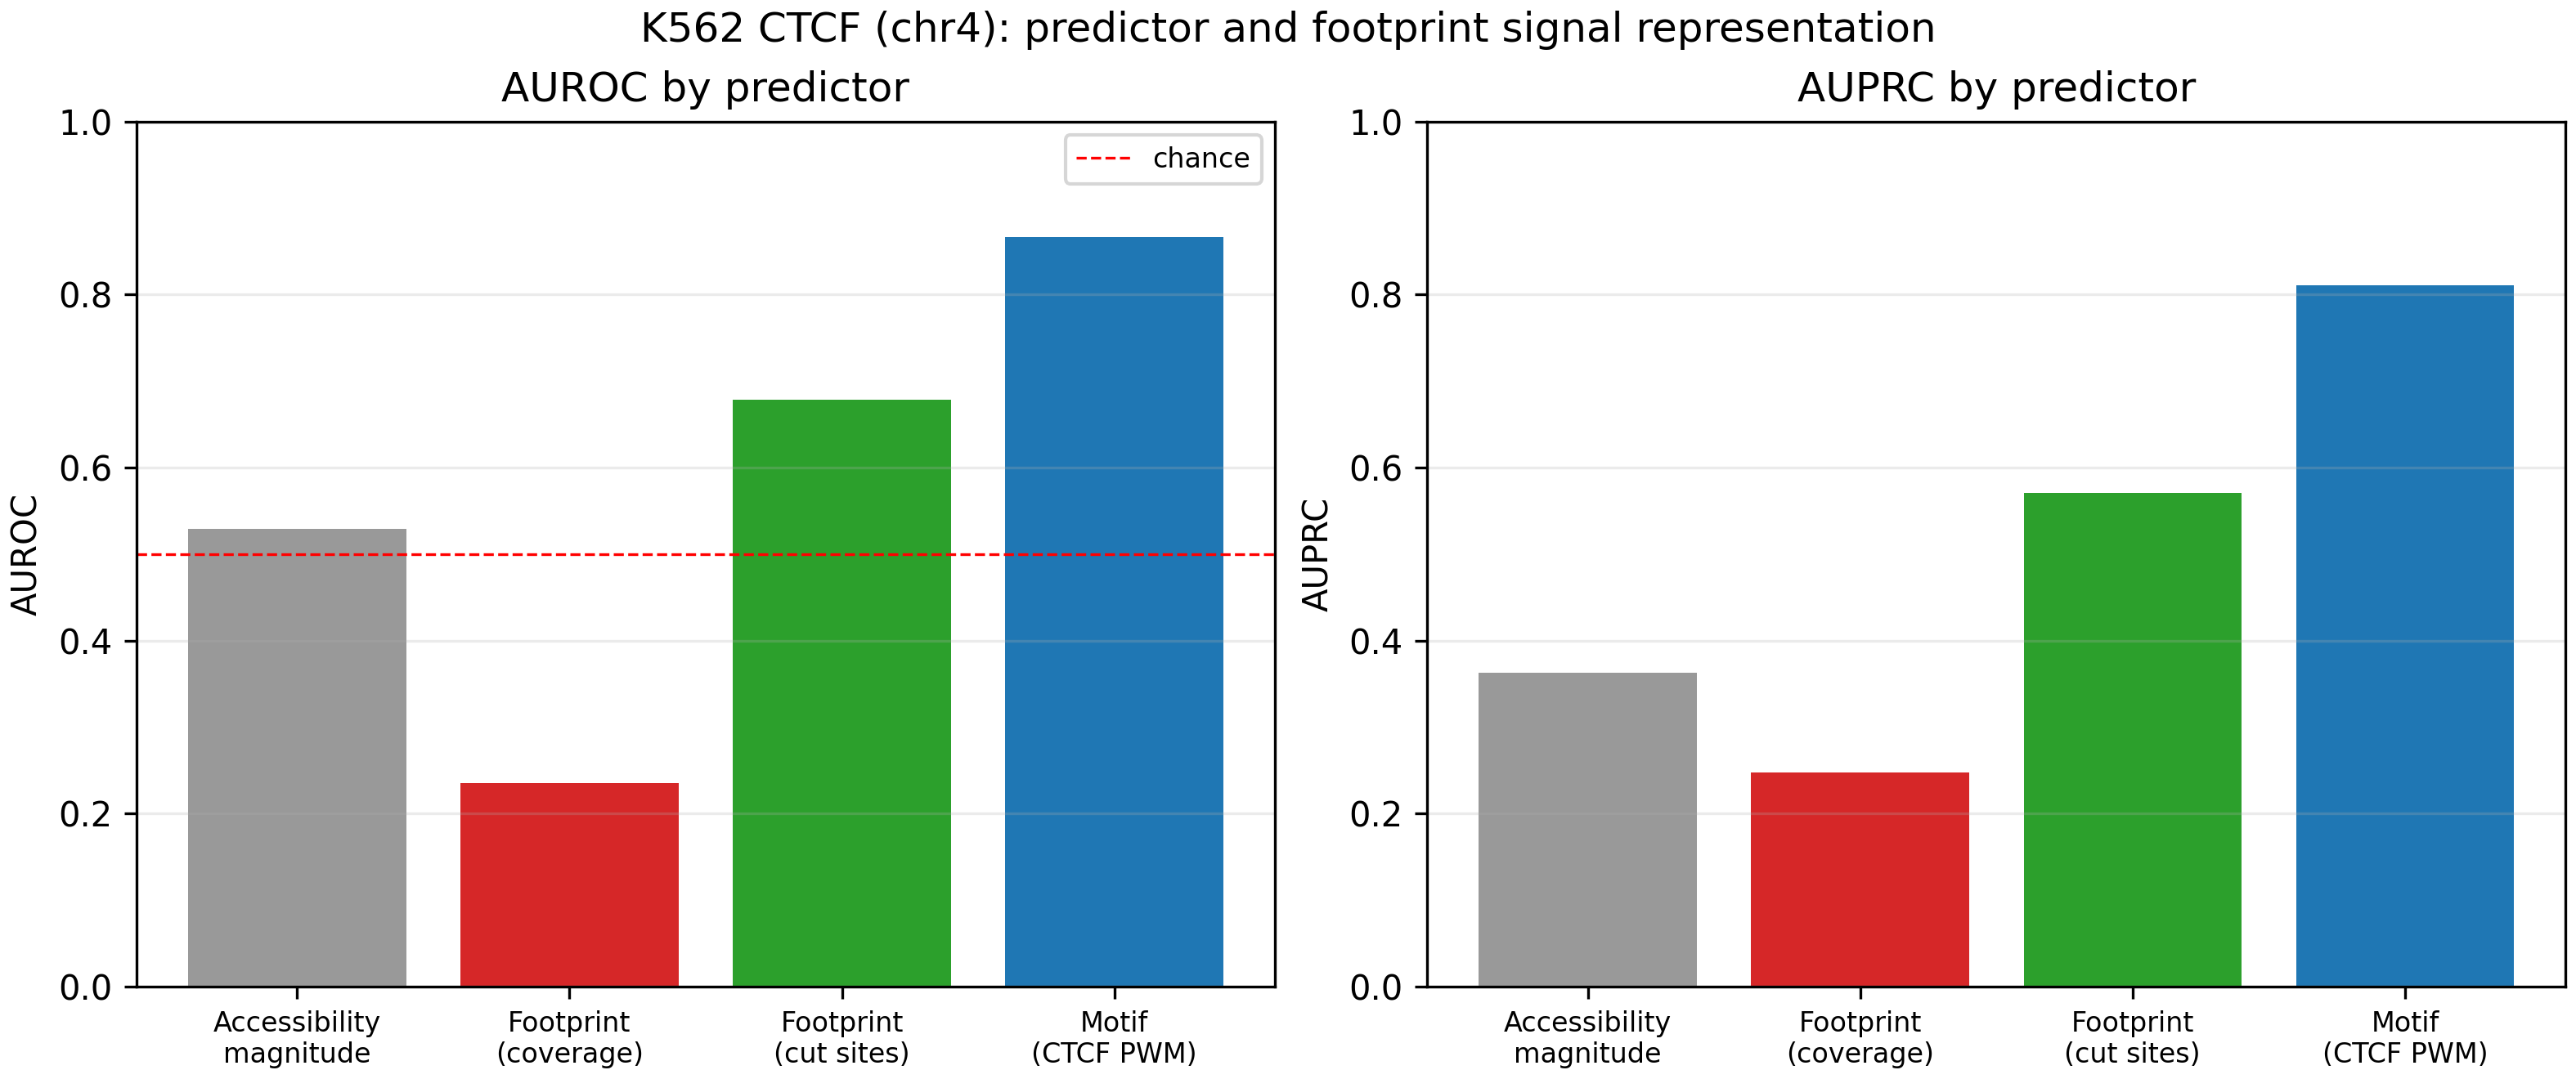
\includegraphics[width=\textwidth]{figures/footprint_representation.png}
\caption{Predictor comparison for K562 CTCF (chromosome~4). A footprint-occupancy
score is informative only at Tn5 cut-site resolution (green, AUROC $0.68$); the same
score on smoothed coverage is inverted and uninformative (red, $0.24$). Raw
accessibility (grey) is near chance and the CTCF motif (blue) is the single
strongest predictor.\label{fig:footprint}}
\end{figure}

%==================================================================
\section{Discussion}
%==================================================================

\texttt{fp-tools} contributes a reproducible platform for classical and
first-version ATAC-seq footprinting workflows. Its comparative strengths are
interface consistency across bias correction, footprint scoring, differential
binding, and aggregate visualization; deterministic regression coverage; explicit
handling of replicate-aware summaries; and an extension model in which multiscale,
de novo motif-preparation, and pseudobulk utilities are opt-in and non-disruptive
(Table~\ref{tab:features}). These properties target the practical friction that
slows applied ATAC-seq analysis and cross-method benchmarking today.

\begin{table}[H]
\caption{Feature comparison across widely used ATAC-seq regulatory-analysis tools.
\checkmark, native first-class support; $\circ$, partial or indirect support;
\textemdash, absent. The \texttt{fp-tools} column covers the first-version scope described in this paper.\label{tab:features}}
\footnotesize
\newcolumntype{C}{>{\centering\arraybackslash}X}
\begin{tabularx}{\textwidth}{Xcccccc}
\toprule
\textbf{Feature} & \textbf{fp-tools} & \textbf{TOBIAS} & \textbf{HINT-ATAC} & \textbf{PRINT/ scPrinter} & \textbf{Chrom- BPNet} & \textbf{maxATAC}\\
\midrule
Bulk ATAC footprinting & \checkmark & \checkmark & \checkmark & \checkmark & $\circ$ & \textemdash\\
Tn5 bias correction & \checkmark & \checkmark & \checkmark & \checkmark & \checkmark & \textemdash\\
Classical footprint scoring & \checkmark & \checkmark & \checkmark & \textemdash & \textemdash & \textemdash\\
Multiscale / nucleosome-aware & \checkmark & \textemdash & $\circ$ & \checkmark & $\circ$ & \textemdash\\
De novo motif discovery & \checkmark & \textemdash & \textemdash & \checkmark & \checkmark & \textemdash\\
scATAC / pseudobulk support & $\circ$ & $\circ$ & $\circ$ & \checkmark & $\circ$ & $\circ$\\
Replicate-aware reporting & \checkmark & $\circ$ & $\circ$ & $\circ$ & \textemdash & \textemdash\\
Visualization / reporting & \checkmark & \checkmark & $\circ$ & \checkmark & \checkmark & $\circ$\\
YAML / batch execution & \checkmark & \textemdash & \textemdash & \textemdash & \textemdash & \textemdash\\
\bottomrule
\end{tabularx}
\end{table}

We do not claim parity with deep sequence-to-profile models on every task where
learned base-resolution sequence features dominate; ChromBPNet-class models and
their attribution-based interpreters are powerful for sequence-driven occupancy and
variant-effect prediction~\cite{chrombpnet2024}. Those models, however, are
computationally heavy---requiring GPU training and large compute budgets---and
their learned enzyme-bias correction is itself incomplete and factor-dependent,
whereas the supported \texttt{fp-tools} first-version workflow emphasizes
lightweight, reproducible classical analyses that are easy to run and audit.
The multiscale and replicate-aware modules are pragmatic additions grounded in the
available signal: in particular, the replicate-aware standard error is
reconstructed from reported $p$-values rather than from per-replicate scores, so it
should be read as a calibrated uncertainty heuristic rather than a full
hierarchical model, and per-replicate inputs would enable a stronger formulation in
future work.

Limitations remain. The present benchmark evaluates discrimination within each
cell--TF task under chromosome-held-out cross-validation; whole-genome
cross-cell-line transfer (training on some cell lines and testing on others) and
direct head-to-head runs of external tools such as TOBIAS, HINT-ATAC, and
ChromBPNet on the identical locus sets are the next steps before broad,
field-relative superiority claims. Larger public-benchmark inputs depend on external data acquisition, intentionally
kept outside version control for size and licensing reasons. Natural next steps
include larger external-tool comparisons, stronger per-replicate statistical
models, and additional public validation datasets.

%==================================================================
\section{Conclusions}
%==================================================================

We presented \texttt{fp-tools}, a standalone, reproducible command-line platform
that unifies classical ATAC-seq footprinting with opt-in multiscale,
motif-discovery-preparation, pseudobulk, and replicate-aware reporting utilities.
By keeping core workflows stable and test-covered while adding new behavior as
composable utilities---and by pairing them with a tiered public-data benchmark and
figure infrastructure---the package lowers the barrier to standardized,
benchmarkable regulatory-genomics analysis. Future work will add larger whole-genome transfer studies, direct external-tool
comparisons, and stronger hierarchical differential-binding validation.

\vspace{6pt}

\authorcontributions{Conceptualization, Y.L. and C.Y.; methodology, Y.L.; software,
Y.L.; validation, Y.L.; formal analysis, Y.L.; investigation, Y.L.; data curation,
Y.L.; writing---original draft preparation, Y.L.; writing---review and editing, Y.L.
and C.Y.; visualization, Y.L.; supervision, C.Y.; project administration, C.Y.;
funding acquisition, C.Y. All authors have read and agreed to the published version
of the manuscript.}

\funding{This research received no external funding.}

\institutionalreview{Not applicable. This study used only publicly available,
de-identified datasets and did not involve new experiments on humans or animals.}

\informedconsent{Not applicable.}

\dataavailability{\texttt{fp-tools} is openly available at
\url{https://github.com/oncologylab/fp-tools}. All benchmark manifests, schemas,
analysis scripts, and figure generators are included in the repository. Public
input datasets are obtained from the ENCODE Project~\cite{encode2012}, the 10x
Genomics PBMC Multiome example~\cite{tenxpbmc2021}, and motif databases (e.g.,
JASPAR~\cite{jaspar2026}) via the included discovery and download scripts.
Manifests, scripts, small result tables, source tables, and figures are stored in
the main repository; large reusable example-data files are distributed separately
through the public \texttt{oncologylab/fp-tools-data} repository release assets,
and full raw public inputs are regenerated from committed manifests rather than
stored in version control.}

\acknowledgments{The author thanks the ENCODE Project Consortium and the
maintainers of the open-source tools referenced in this work for making their data
and software publicly available.}

\conflictsofinterest{The author declares no conflicts of interest.}

%==================================================================
\bibliography{references}

\end{document}
